\documentclass[xcolor=dvipsnames]{beamer}
\makeatletter\def\Hy@xspace@end{}\makeatother
\usepackage{graphicx, color, amssymb, amsmath, bm, rotating, graphics,
epsfig, multicol, amsthm}
\usepackage[english]{babel}
\usepackage[T1]{fontenc}
\usepackage[ansinew]{inputenc}
\usepackage[authoryear]{natbib}
%\newcommand{\newblock}{}  %needed to make beamer and natbib play nice
\usepackage{tikz}
%\usetheme{Boadilla}
%\usecolortheme{lily}
 \usecolortheme[named=Red]{structure}
% \setbeamercolor{structure}{bg=black}
% \setbeamercolor{structure}{fg=Goldenrod}
% \setbeamercolor{title}{bg=Black}
% \setbeamercolor{frametitle}{bg=Black, fg=Goldenrod}
% \setbeamercolor{title in head/foot}{fg=Black, bg=Goldenrod}
% \setbeamercolor{author in head/foot}{fg=Goldenrod, bg=Black}
% \setbeamercolor{institute in head/foot}{fg=Goldenrod, bg=Black}
% \setbeamercolor{date in head/foot}{fg=Goldenrod, bg=Black}
\setbeamercovered{transparent=0}
\beamertemplatenavigationsymbolsempty

\title[Intro to Stan]{Introduction to Stan for \\
Markov Chain Monte Carlo}
\date{April 25, 2017}

%\subtitle{}
\author[Matt Simpson]{Matthew Simpson}
\institute[Mizzou Statistics]{Department of Statistics, University of Missouri}

\begin{document}

\begin{frame}[fragile]
\titlepage

These slides and accompanying \verb0R0 and Stan files are available at \url{http://stsn.missouri.edu/education-and-outreach.shtml}
\end{frame}

% \begin{frame}[fragile]
% \frametitle{Abstract}
% \centering
% In the first part of this talk I introduce Hamiltonian Monte Carlo (HMC) and its implementation in Stan. The focus is on building intuition and not on theory, e.g. for how HMC works, how Stan solves many of the problems typically associated with implementing HMC, and for why HMC and Stan are attractive alternatives to Gibbs based sampling algorithms. In the second part of the talk, I provide a brief introduction to using Stan with the \verb0rstan0 \verb0R0 package. I provide several examples in this portion of the talk, guidance for interpreting Stan's warning and error messages, and intuition for how to construct better HMC samplers using Stan.
% \end{frame}

\begin{frame}
\frametitle{Stan is...}

\begin{columns}[c]
 \begin{column}[c]{0.5\textwidth}

\begin{itemize}
\item[]
\begin{center}
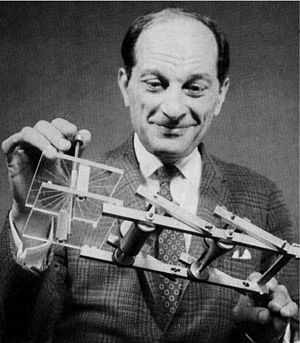
\includegraphics[width=0.5\textwidth]{stan.jpg}
\end{center}
\end{itemize}
\end{column}

\begin{column}[c]{0.5\textwidth}
\begin{itemize}
\item[] \textbf{Stanislaw Ulam}, inventor of Monte Carlo methods.\\
\end{itemize}
\end{column}
\end{columns}

\vspace{0.2cm}

\begin{itemize}
\item[] \url{http://mc-stan.org/}

\vspace{0.2cm}

\item[] A \textbf{probabilistic programming language} that implements {\color{red}\textbf{Hamiltonian Monte Carlo (HMC)}}, variational Bayes, and (penalized) maximum likelihood estimation.\\

\vspace{0.2cm}

\item[] Available on Linux, Mac, and Windows with interfaces in \textbf{R}, \textbf{Python}, shell (command line), MATLAB, Julia, Stata, and Mathematica.

\end{itemize}
\end{frame}

\begin{frame}
\frametitle{Markov chain Monte Carlo (MCMC)}
Goal: sample from some target density ${\color{blue}\pi(\bm{q})}$.\\

\vspace{0.5cm}

Create a Markov chain with Markov transition density $k(\bm{q}'|\bm{q})$.
\begin{itemize}
\item Start with arbitrary $\bm{q}^{(0)}$ and repeatedly sample $\bm{q}^{(i+1)} \sim k(\bm{q}'|\bm{q}^{(i)})$.\\

\vspace{0.2cm}

\item Under easy conditions the chain is {\color{red}ergodic}, $\bm{q}^{(i)} \to {\color{blue}\pi(\bm{q})}$, and
\begin{align*}
  \frac{1}{N}\sum_{i=1}^N f(\bm{q}^{(i)}) \to \mathrm{\color{blue}E}_{\color{blue}\pi}[f(\bm{q})]&& \mbox{ almost surely.}
\end{align*}

\vspace{0.2cm}

\item Additionally if the chain is {\color{red}geometrically ergodic}:
\begin{align*}
  \frac{1}{N}\sum_{i=1}^N f(\bm{q}^{(i)}) \to \mathrm{N}\left(\mathrm{\color{blue}E}_{\color{blue}\pi}[f(\bm{q})], \frac{\mathrm{\color{blue}var}_{\color{blue}\pi}[f(\bm{q})]}{ESS}\right).
\end{align*}
\end{itemize}
\end{frame}

\begin{frame}
\frametitle{HMC in Theory}
Let ${\color{blue}\pi(\bm{q})}>0$ for all ${\bm{q}}\in\Re^n$. Construct auxillary variable $\bm{p}\in\Re^n$.
\begin{itemize}
\item[] $V({\bm{q}})\phantom{,\bm{p}} = -\log {\color{blue}\pi(\bm{q})}$ --- \emph{potential energy}.
\item[] $T({\bm{q}}, \bm{p}) = - \log \pi(\bm{p} | {\bm{q}})$ --- \emph{kinetic energy}.
\item[] $H({\bm{q}}, \bm{p}) = V({\bm{q}}) + T({\bm{q}}, \bm{p})$ --- \emph{Hamiltonian}, total energy.
\end{itemize}
where ${\bm{q}}$ denotes {\color{red}\emph{position}} and $\bm{p}$ denotes {\color{red}\emph{momentum}}.

\vspace{0.3cm}

Energy-preserving evolution in time is defined by Hamilton's equations:
\begin{align*}
\frac{\mathrm{d}\bm{p}}{\mathrm{d} t} = - \frac{\partial H}{\partial {\bm{q}}}; && \frac{\mathrm{d}{\bm{q}}}{\mathrm{d} t} = + \frac{\partial H}{\partial \bm{p}}.
\end{align*}
How to implement HMC in theory:
\begin{enumerate}
\item Sample momenta variables: $\bm{p}' \sim \pi(\bm{p}|\bm{q}^{(i)})$.
\item Run Hamiltonian evolution forward in time from $(\bm{q}^{(i)}, \bm{p}')$ for a some amount of {\color{red}\emph{integration time}} to obtain $(\bm{q}^{(i+1)}, \bm{p}^{(i+1)})$.
\end{enumerate}
\end{frame}

\begin{frame}
\frametitle{HMC in Pictures}
\begin{center}
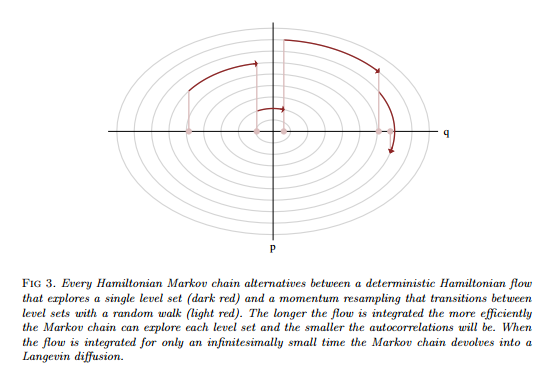
\includegraphics[height=0.5\textheight]{hmc.png}
\end{center}

HMC samples a level set, then moves along that set.\\~\\


Long integration time $\implies$ $\approx$ zero autocorrelation in the chain.\\~\\

{\footnotesize Picture from \textbf{Identifying the Optimal Integration Time in HMC}\\ (Michael Betancourt)
\url{https://arxiv.org/pdf/1601.00225.pdf}}
\end{frame}

\begin{frame}[fragile]
\frametitle{HMC in Practice}
To implement HMC for a \textbf{differentiable} target ${\color{blue}\pi(\bm{q})}$ you need:
\vspace{0.2cm}
\begin{enumerate}
\item No discrete valued parameters in $\bm{q}$.
\begin{itemize}
\item Usually can integrate them out, e.g. mixture models.
\end{itemize}
\vspace{0.2cm}
\item No constrained parameters in $\bm{q}$.
\begin{itemize}
\item Stan: transform and compute the log-Jacobian automatically.
\end{itemize}
\vspace{0.2cm}
\item The gradient vector of $\log {\color{blue}\pi(\bm{q})}$.
\begin{itemize}
\item Stan: use C++ autodiff library to do this automatically and accurately.
\end{itemize}
\vspace{0.2cm}
\item Choose a kinetic energy, i.e. $\pi(\bm{p}|\bm{q})$.
\begin{itemize}
\item Stan: $\mathrm{N}(\bm{0}, \bm{M})$ and tune $\bm{M}$ during warmup. (Euclidean HMC)
\item More intelligent: $\bm{M}(\bm{q})$. (Riemannian HMC; future Stan)
\end{itemize}
\end{enumerate}
\begin{align*}
{\color{red}\Huge{\vdots}}
\end{align*}
\end{frame}

\begin{frame}
\frametitle{HMC in Practice (continued)}
To implement HMC for a \textbf{differentiable} target ${\color{blue}\pi(\bm{q})}$ you need:
\vspace{0.2cm}
\begin{enumerate}
\item[5.] Numerical integrator for Hamilton's equations.
\begin{itemize}
\item Need to make an adjustment to the Hamiltonian flow and use a Metropolis correction to ensure detailed balance.
\vspace{0.2cm}
\item Use leapfrog integration $\implies$ how many leapfrog steps?
\vspace{0.2cm}
\item Stan: adapt number of leapfrog steps to hit a target Metropolis acceptance rate --- default is 80\%.
\end{itemize}
\vspace{0.2cm}
\item[6.] An integration time. How long is long enough?
\begin{itemize}
\item Old Stan: No U-Turn Criterion / No U-Turn Sampler (NUTS) \\
\vspace{0.2cm}
``stop when we start heading back toward where we started.''
\vspace{0.2cm}
\item New Stan: eXhaustive HMC (XHMC/XMC/better NUTS) \\
\vspace{0.2cm}
``stop when it looks like autocorrelation should be low.''
\vspace{0.2cm}
\end{itemize}
\end{enumerate}
\end{frame}

\begin{frame}
\frametitle{Why Hamiltonian Monte Carlo?}

The long answer:
\begin{itemize}
\item \textbf{Everything You \emph{Should} Have Learned About MCMC} \\
(Michael Betancourt) \\
\url{https://www.youtube.com/watch?v=DJ0c7Bm5Djk&feature=youtu.be&t=4h40m10s}
\item \textbf{A Conceptual Introduction to HMC} (Michael Betancourt) \\
\url{https://arxiv.org/pdf/1701.02434.pdf}
\item \textbf{Hamiltonian Monte Carlo for Hierarchical Models}
(Michael Betancourt and Mark Girolami) \\
\url{https://arxiv.org/pdf/1312.0906.pdf}
\end{itemize}

\vspace{0.5cm}

The short answer:
\begin{itemize}
\item Works in high dimensions.
\item More robust.
\item Makes noise when it fails.
\end{itemize}

\end{frame}

\begin{frame}
\frametitle{Works in high dimensions}
Probability mass is concentrated on the \emph{\textbf{\color{red} typical set}}
\begin{itemize}
\item the smallest volume set with $1 - \epsilon$ probability.\\~\\
\end{itemize}
\begin{center}
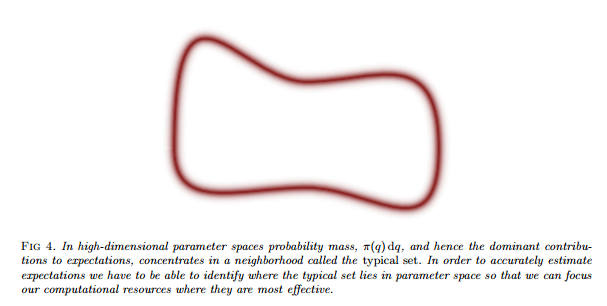
\includegraphics[height=0.4\textheight]{typicalset.png}
\end{center}
In high dimensions, this is a thin shell \emph{around} the mode.
\begin{itemize}
\item Random walk methods have to take tiny steps.
\item Gibbs methods take a long time to move around the surface.
\item Modes are far from mass $\to$ mode-based methods may fail.
\item HMC moves \emph{around} the typical set.
\end{itemize}
\end{frame}

\begin{frame}
\frametitle{Intuition for the Typical Set}
Typical set: smallest volume set with $1 - \epsilon$ probability.\\~\\

Why is it a shell? Concentration of measure.
\begin{itemize}
\item Given $n$ random variables, it is unlikely for all of them to be near their respective typical values when $n$ is large.\\~\\
\end{itemize}

Consider $z_i \stackrel{iid}{\sim} \mathrm{N}(0, 1)$, $i = 1,2,\dots, n$; $\bm{z} = (z_1,z_2,\dots,z_n)$.
\begin{itemize}
\item The distance between $\bm{z}$ and its mode is $d = \sqrt{\sum_{i=1}^nz_i^2}$.
\item $d^2\sim\chi^2_n$ and $d\sim\chi_n$.
\end{itemize}
\begin{center}
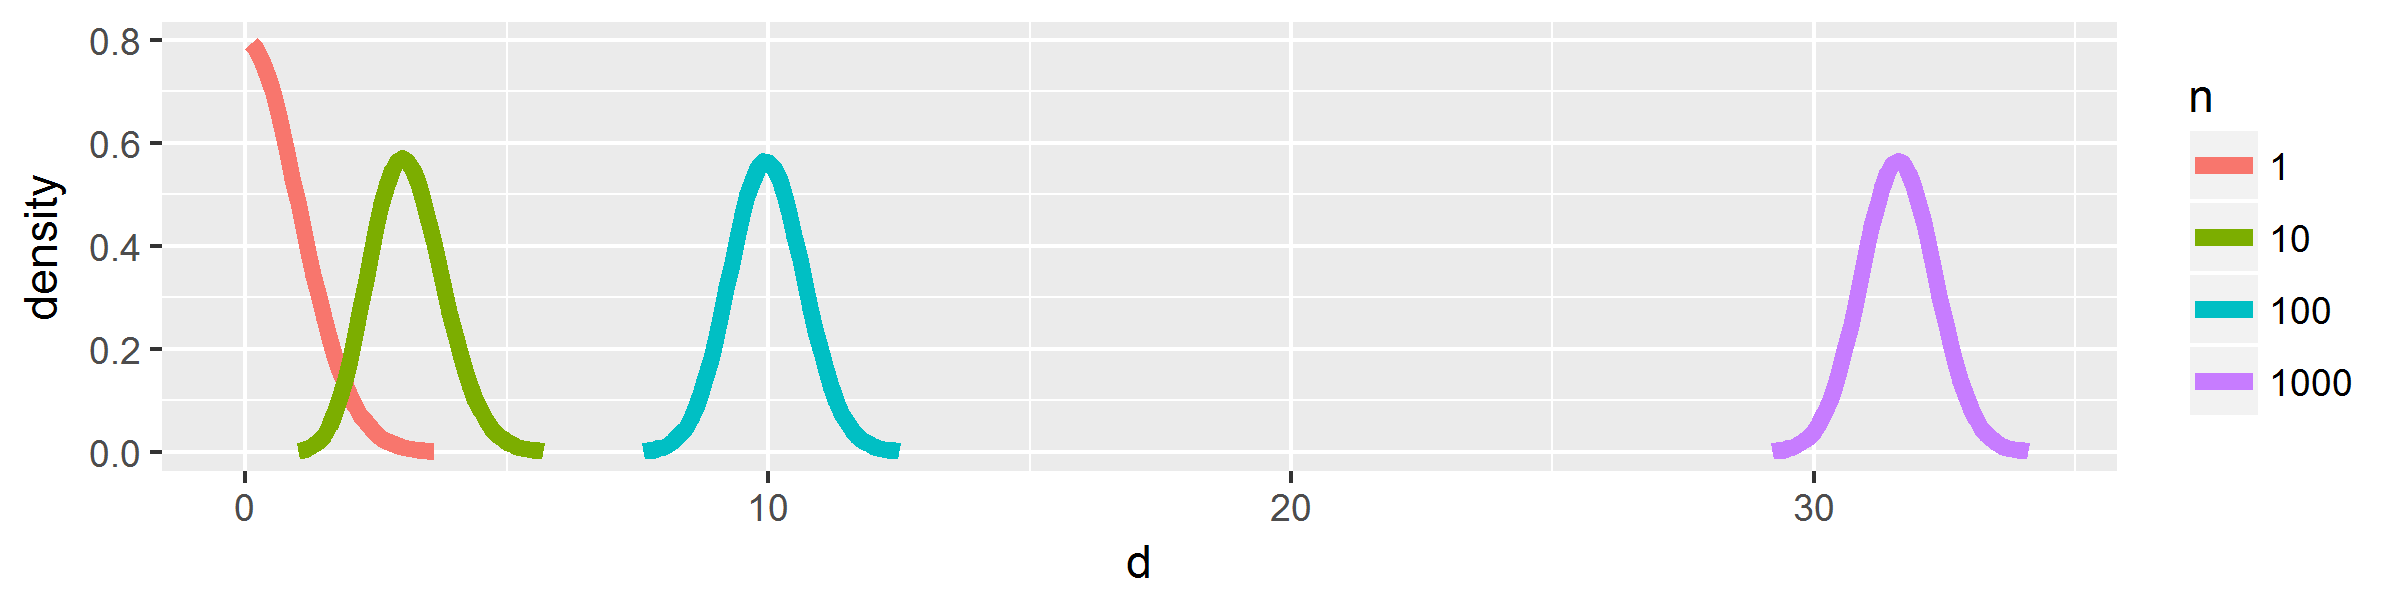
\includegraphics[width = \textwidth]{code/chiplot.png}
\end{center}
More: {\scriptsize \url{http://mc-stan.org/documentation/case-studies/curse-dims.html}}
\end{frame}

\begin{frame}
\frametitle{Robustness and Noisy Failure}
HMC has guaranteed geometric ergodicity in a larger class of target densities than alternatives. {\scriptsize \url{https://arxiv.org/pdf/1601.08057.pdf} \\\textbf{On the Geometric Ergodicity of HMC} (Ligingstone, Betancourt, et. al.) }

\vspace{0.5cm}

When geometric ergodicity fails, HMC often won't sample due to numerically infinite gradients (``divergent transitions'').
\begin{center}
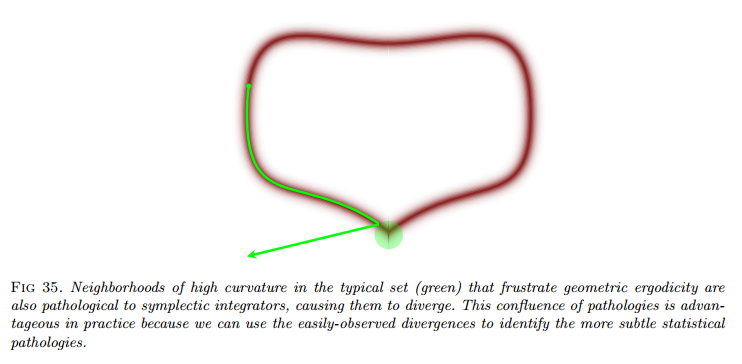
\includegraphics[height = 0.4\textheight]{divergent.png}
\end{center}
\begin{itemize}
\item Caused by weird posterior geometries.
\item Common in hierarchical models.
\item Also a problem in Gibbs samplers, but they still give output.
\end{itemize}
\end{frame}

\begin{frame}[fragile]
\frametitle{Using Stan: Resources}
How to install Stan and \verb0rstan0 (Follow the directions carefully!):
\begin{itemize}
\item \url{https://github.com/stan-dev/rstan/wiki/RStan-Getting-Started}
\end{itemize}

Stan manual (it's very good and constantly being improved):
\begin{itemize}
\item \url{https://github.com/stan-dev/stan/releases/download/v2.14.0/stan-reference-2.14.0.pdf}
\end{itemize}

Links to the manual, examples, tutorials, and case studies:
\begin{itemize}
\item \url{http://mc-stan.org/documentation/}
\end{itemize}

\verb0rstan0 documentation:
\begin{itemize}
\item \url{http://mc-stan.org/interfaces/rstan.html}
\end{itemize}

A brief guide to Stan's warnings:
\begin{itemize}
\item \url{http://mc-stan.org/misc/warnings.html}
\end{itemize}

A shorter intro with a different emphasis:
\begin{itemize}
\item \url{http://mlss2014.hiit.fi/mlss_files/2-stan.pdf}
\end{itemize}
\end{frame}

\begin{frame}[fragile]
\frametitle{Using Stan: A Simple Example}
Running example: regression with observation errors.\\~\\

Generative model for fake data:
\begin{align*}
y_i \stackrel{ind}{\sim} \mathrm{N}(\theta_i, s_i^2), && \theta_i \stackrel{ind}{\sim} \mathrm{N}(\alpha + \bm{x}_i'\bm{\beta}, \sigma^2) && \mbox{ for } i=1,2,\dots,N.
\end{align*}
From \verb0stanintro.R0:

{\tiny
\begin{verbatim}
n <- 100
alpha <- 150
beta <- c(0.05, 100, -.003)
x <- cbind(runif(n, -100, 100), rnorm(n, 10, 1/10), rgamma(n, 1, 1/100))
sigma <- 10
standard.errors <- rep(10*sigma, n)
theta <- rnorm(n, alpha + x%*%beta, sigma)
y <- rnorm(n, theta, standard.errors)
\end{verbatim}
}


Regression model ignoring observation errors:
\begin{align*}
y_i \stackrel{ind}{\sim} \mathrm{N}(\alpha + \bm{x}_i'\bm{\beta}, \sigma^2) && \mbox{ for } i=1,2,\dots,N
\end{align*}
with independent priors:
\begin{align*}
\alpha \sim \mathrm{T}_1(100, 1000^2), && \beta_k&\stackrel{iid}{\sim} \mathrm{N}(10, 100^2), &&\sigma \sim \mathrm{half-T}_{5}(0, 100^2).
\end{align*}
\end{frame}


\begin{frame}[fragile]
\frametitle{Using Stan: A Simple Example}
Define the model in a \verb0.stan0 file, e.g. \verb0regression.stan0:
{\tiny
\begin{verbatim}
data {
  int<lower = 1> n_obs;
  int<lower = 1> n_cov;
  vector[n_obs] y;
  matrix[n_obs, n_cov] x;
  real beta_prior_mn;
  real<lower = 0> beta_prior_sd;
  real alpha_prior_loc;
  real<lower = 0> alpha_prior_scale;
  real<lower = 0> sig_prior_scale;
  real<lower = 0> sig_prior_df;
}
parameters {
  real alpha;
  vector[n_cov] beta;
  real<lower = 0> sigma;
}
model {
  y ~ normal(alpha + x*beta, sigma);
  alpha ~ cauchy(alpha_prior_loc, alpha_prior_scale);
  beta ~ normal(beta_prior_mn, beta_prior_sd);
  sigma ~ student_t(sig_prior_df, 0, sig_prior_scale);
}
\end{verbatim}
}
\end{frame}

\begin{frame}[fragile]
\frametitle{The .stan File}
Defines a target density as a function of data and parameters.
\begin{itemize}
\item Data: all things that are fixed during MCMC, including prior hyperparameters and what we normally think of as ``data''.
\item Parameters: all things we want/need to sample from.\\~\\
\end{itemize}
The file is composed of several ``program blocks'' in a specific order.
\vspace{-.5cm}
\begin{itemize}
\item ``parameters'' and ``model'' blocks are mandatory.
\item ``data'' block is necessary to read data into Stan.
\item And several others.
\end{itemize}
\begin{verbatim}
data {
  // define all variables to be read into Stan here
}
parameters {
  // define all parameters of the target density here
}
model {
  // define model as a function parameters and data here
}
\end{verbatim}
\end{frame}


\begin{frame}[fragile]
\frametitle{Defining variables}
A variable can be defined at the beginning of any block,\\
or at the beginning of any code chunk (\verb0{...}0).\\~\\
\begin{itemize}
\item Stan has two basic data types: \verb0int0 and \verb0real0.
\item Vectors and matrices are collections of \verb0real0s.
\item Can define arrays of \verb0int0s or \verb0real0s... or vectors or whatever.
\item Must define every variable that Stan will use.
\item Arrays, vectors, and matrices must have defined dimensions.
\item Can (and should) specify any relevant bounds for all variables (error checking \& more).\\~\\
\end{itemize}
Basic syntax: \verb0int n;0 or \verb0real y;0.
\end{frame}

\begin{frame}[fragile]
\frametitle{Some example variable definitions}
\begin{verbatim}
int<lower = 1> A;  // A >= 1 (constraints are inclusive)
real<upper = 0> B; // B <= 0
real<lower = 0, upper = 1> C; // 0 <= C <= 1
vector[10] D;                 // vector of 10 reals
vector<lower = 0>[10] E;      // vector of 10 reals >= 0
row_vector[5] F;              // row vector of 5 reals
matrix[10, 5] H;              // 10x5 matrix of reals
cov_matrix I[2];              // 2x2 PD matrix
corr_matrix J[2];             // 2x2 PD matrix
cholesky_factor_cov K[2];     // lower triangular
cholesky_factor_corr L[2];    // lower triangular
simplex M[5]; // each 0 < M[i] < 1; sum_i M[i] = 1
\end{verbatim}
Note: \verb0C0-style syntax: end statements with a semicolon (\verb0;0),\\
\ \ \ \ \ \ \ \, and `\verb0//0' comments the rest of the line (like \verb0#0 in \verb0R0).
\end{frame}

\begin{frame}[fragile]
\frametitle{Array / matrix indexing: mostly like R}
Indexing order: array dimensions, then row, then column.
\begin{verbatim}
real A[N];         // N-dim array
vector[N] B;       // N-dim vector
matrix[N, M] C;    // NxM matrix
vector[N] D[M];    // M N-dim vectors
matrix[N, M] E[K]; // K NxM matrices
A[3]; B[3];        // access 3rd element
A[1:3]; B[1:3];    // 1st - 3rd elements
A[ii]; B[ii]; // if ii = [1, 3], 1st and 3rd elements
C[1,2];            // 1st row / 2nd column
D[1,2];            // 2nd element of 1st vector
C[1];              // first row
D[1];              // first vector
C[,1];             // first column
D[,1];             // vector of 1st elements
E[1,1:4,1:4];      // top left 4x4 submatrix of 1st matrix
\end{verbatim}
...and combinations of the above.
\end{frame}

\begin{frame}[fragile]
\frametitle{Data block}
Define all data that will be read into Stan. \verb0regression.stan0:
\begin{verbatim}
data {
  int<lower = 1> n_obs;
  int<lower = 1> n_cov;
  vector[n_obs] y;
  matrix[n_obs, n_cov] x;
  real beta_prior_mn;
  real<lower = 0> beta_prior_sd;
  real alpha_prior_loc;
  real<lower = 0> alpha_prior_scale;
  real<lower = 0> sigma_prior_scale;
  real<lower = 0> sigma_prior_df;
}
\end{verbatim}
This block \emph{only} consists of variable definitions.\\~\\

Any constraints are checked once before the sampler is run.
\end{frame}

\begin{frame}[fragile]
\frametitle{Parameters block}
Define all parameters in the model. \verb0regression.stan0:
\begin{verbatim}
parameters {
  real alpha;
  vector[n_cov] beta;
  real<lower = 0> sigma;
}
\end{verbatim}
This block \emph{only} consists of variable definitions.\\~\\

Stan automatically transforms constrained parameters to unconstrained Euclidean space and computes the relevant Jacobian. \vspace{-.5cm}
\begin{itemize}
\item Stan can hand simple constraints stated in terms of lower \& upper bounds, e.g. \verb0real<lower = mu_x> mu_y;0,
\item ...and certain hardcoded complex constraints, e.g. covariance and correlation matrices, Cholesky factors of both, etc.
\end{itemize}
\end{frame}

\begin{frame}[fragile]
\frametitle{Model block}
Define the model in terms of parameters and data. \verb0regression.stan0:
\begin{verbatim}
  y ~ normal(alpha + x*beta, sigma);
  alpha ~ cauchy(alpha_prior_loc, alpha_prior_scale);
  beta ~ normal(beta_prior_mn, beta_prior_sd);
  sigma ~ student_t(sigma_prior_df, 0, sigma_prior_scale);
\end{verbatim}
Each sampling statement (`$\sim$') defines a log-density for the LHS variable. The sum of these log-densities is the target log-density.\\~\\

\textbf{\color{red}The LHS must \emph{NOT} be a nonlinear transformation of parameters. If it is, you need the Jacobian.}
\begin{itemize}
\item Better to write the model in a way that does not use a transformation on the LHS of a sampling statement.\\~\\
\end{itemize}

Note: \verb0sigma0 is defined to be $\geq 0$ in the parameters block.
\begin{itemize}
\item Stan handles the normalizing constant from the truncation.
\end{itemize}
\end{frame}

\begin{frame}[fragile]
\frametitle{Arithmetic operators}
`\verb0*0' is matrix multiplication when its arguments are not scalars. Similarly `\verb0/0' and `\verb0\0' are matrix division:
\begin{align*}
A * B = AB, && A / B = AB^{-1}, && A \backslash B = A^{-1}B
\end{align*}
Use `\verb0 .* 0' and `\verb0 ./ 0' for elementwise operations.\\
\ \ \ \ ...but give these operators some space:\\
\ \ \ \ \verb0A.*B0 will throw an error, \verb0A .* B0 will not.\\~\\

Otherwise, most things work just like \verb0R0, except Stan is finicky about dimensions matching (this is good for catching errors).
\begin{itemize}
\item other differences: \verb0||0 for `or', \verb0&&0 for `and', \verb0X'0 for $X$ transpose.\\~\\
\end{itemize}

Check the manual for efficient specialized functions for many common linear algebra (and other) operations, e.g.:
\begin{verbatim}
crossprod(); tcrossprod(); dot_product(); quad_form();
\end{verbatim}
\end{frame}

\begin{frame}[fragile]
\frametitle{Vectorization vs loops}
Sampling statements are vectorized when it makes sense.\\~\\

I.e. the following are equivalent ways of coding $y$'s model:
\begin{itemize}
\item \verb0y ~ normal(alpha + x*beta, sigma);0\
\item
\begin{verbatim}
for(i in 1:n_obs){ // same as in R
  y[i] ~ normal(alpha + x[i]*beta, sigma);
}
\end{verbatim}
\end{itemize}
Stan is written in \verb0C++0 so for loops are fast...\\~\\

But the \verb0autodiff0 library is much faster on vectorized models.
\begin{itemize}
\item Much faster gradient computations.
\item Sampling is cheaper per-iteration (per-leapfrog step).\\~\\
\end{itemize}

Upshot: vectorize wherever you can (see manual).
\end{frame}

\begin{frame}[fragile]
\frametitle{Fitting the model in R}
Fitting a regression:
{\footnotesize
\begin{verbatim}
library(rstan)

## create list of all variables in the data block
regdat <- list(n_obs = n, n_cov = length(beta), y = y, x = x,
               alpha_prior_loc = 100, alpha_prior_scale = 1000,
               beta_prior_mn = 10, beta_prior_sd = 100,
               sigma_prior_df = 5, sigma_prior_scale = 100)

## initialize the model; takes 15-30 seconds
regfit0 <- stan("regression.stan", data = regdat, chains = 1, iter = 1)
## ignore compiler warnings

## sample the model
regfit <- stan(fit = regfit0, data = regdat, cores = 4, chains = 4,
              warmup = 2000, iter = 4000, open_progress = FALSE)
## about 3 minutes to fit per chain
\end{verbatim}
}
\end{frame}

\begin{frame}[fragile]
\frametitle{The stan() function in rstan}
Required arguments:
\begin{itemize}
\item A model --- ``.stan'' file, or \verb0fit = stanfit0, a \verb0stan0 object.
\item data --- list of all variables in the data block of the model.\\
\ \ \ \ \ \ \ \ \ \ \        (only required if the model has a data block)\\~\\
\end{itemize}
Useful named arguments and their defaults:
\begin{itemize}
\item \verb0cores = 10 --- number of cores to use.
\begin{itemize}
\item Parallelizes \emph{across} chains, not within.
\end{itemize}
\item \verb0chains = 40 --- number of chains.
\item \verb1iter = 40001 --- total number of iterations per chain.
\item \verb0warmup = iter/20 --- iterations used for tuning / burn-in.\\~\\
\end{itemize}
Starting values, tuning, etc., taken care of automatically, but much of this is exposed in \verb0stan()0.
\end{frame}

\begin{frame}[fragile]
\frametitle{Running stan()}
\begin{verbatim}
> regfit0 = stan("regression.stan", data = regdat,
+                chains = 1, iter = 1)
...
warning: "BOOST_NO_CXX11_RVALUE_REFERENCES" redefined
...
\end{verbatim}
\begin{itemize}
\item Ignore compiler warnings like the one above.
\end{itemize}
\begin{verbatim}
> regfit = stan(fit = regfit0, data = regdat, cores = 4,
+          chains = 4, warmup = 2000, iter = 4000)
...
Chain 4, Iteration: 4000 / 4000 [100%]  (Sampling)
 Elapsed Time: 79.7899 seconds (Warm-up)
               96.0802 seconds (Sampling)
               175.87 seconds (Total)
\end{verbatim}
\end{frame}

\begin{frame}[fragile]
\frametitle{Traceplots}
\verb0> traceplot(regfit, pars = c("alpha", "beta"))0
\begin{center}
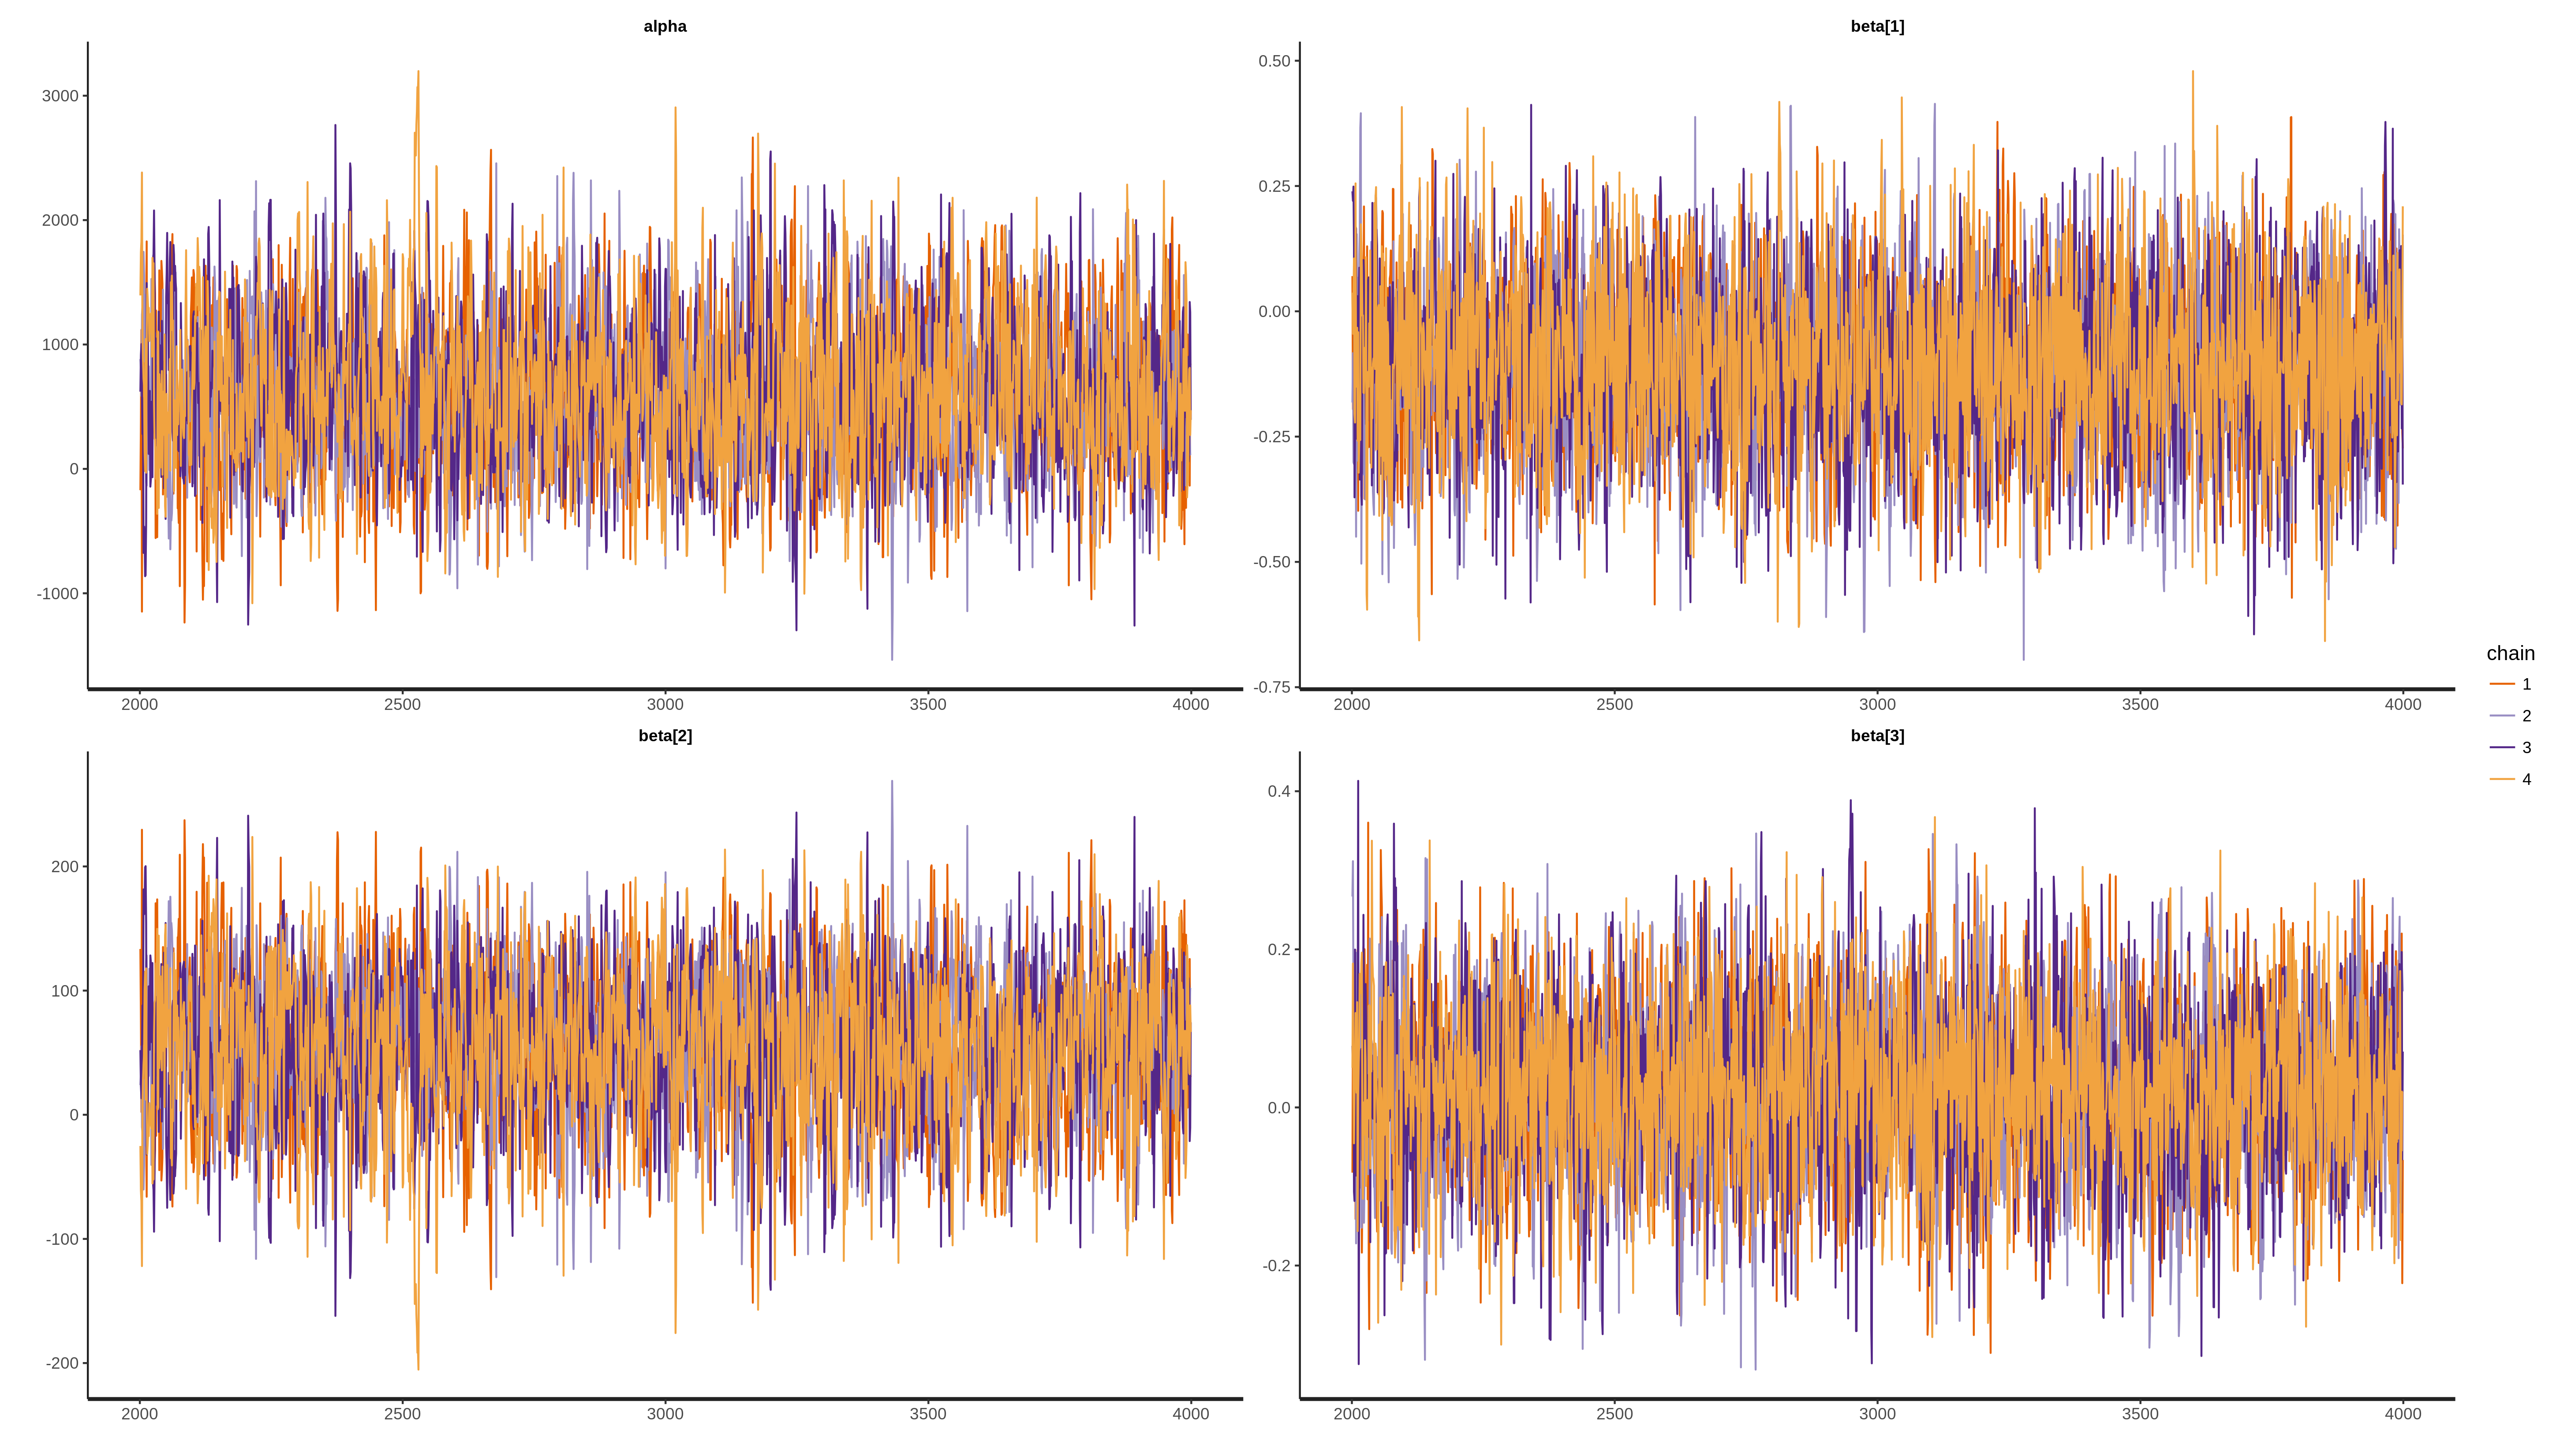
\includegraphics[width = 0.99\textwidth]{code/traceplot1.png}
\end{center}
\end{frame}

\begin{frame}[fragile]
\frametitle{More Traceplots}
{\tiny
\begin{verbatim}
> traceplot(regfit, pars = c("alpha", paste("beta[", 1:2, "]", sep=""), "sigma"))
\end{verbatim}
}
\begin{center}
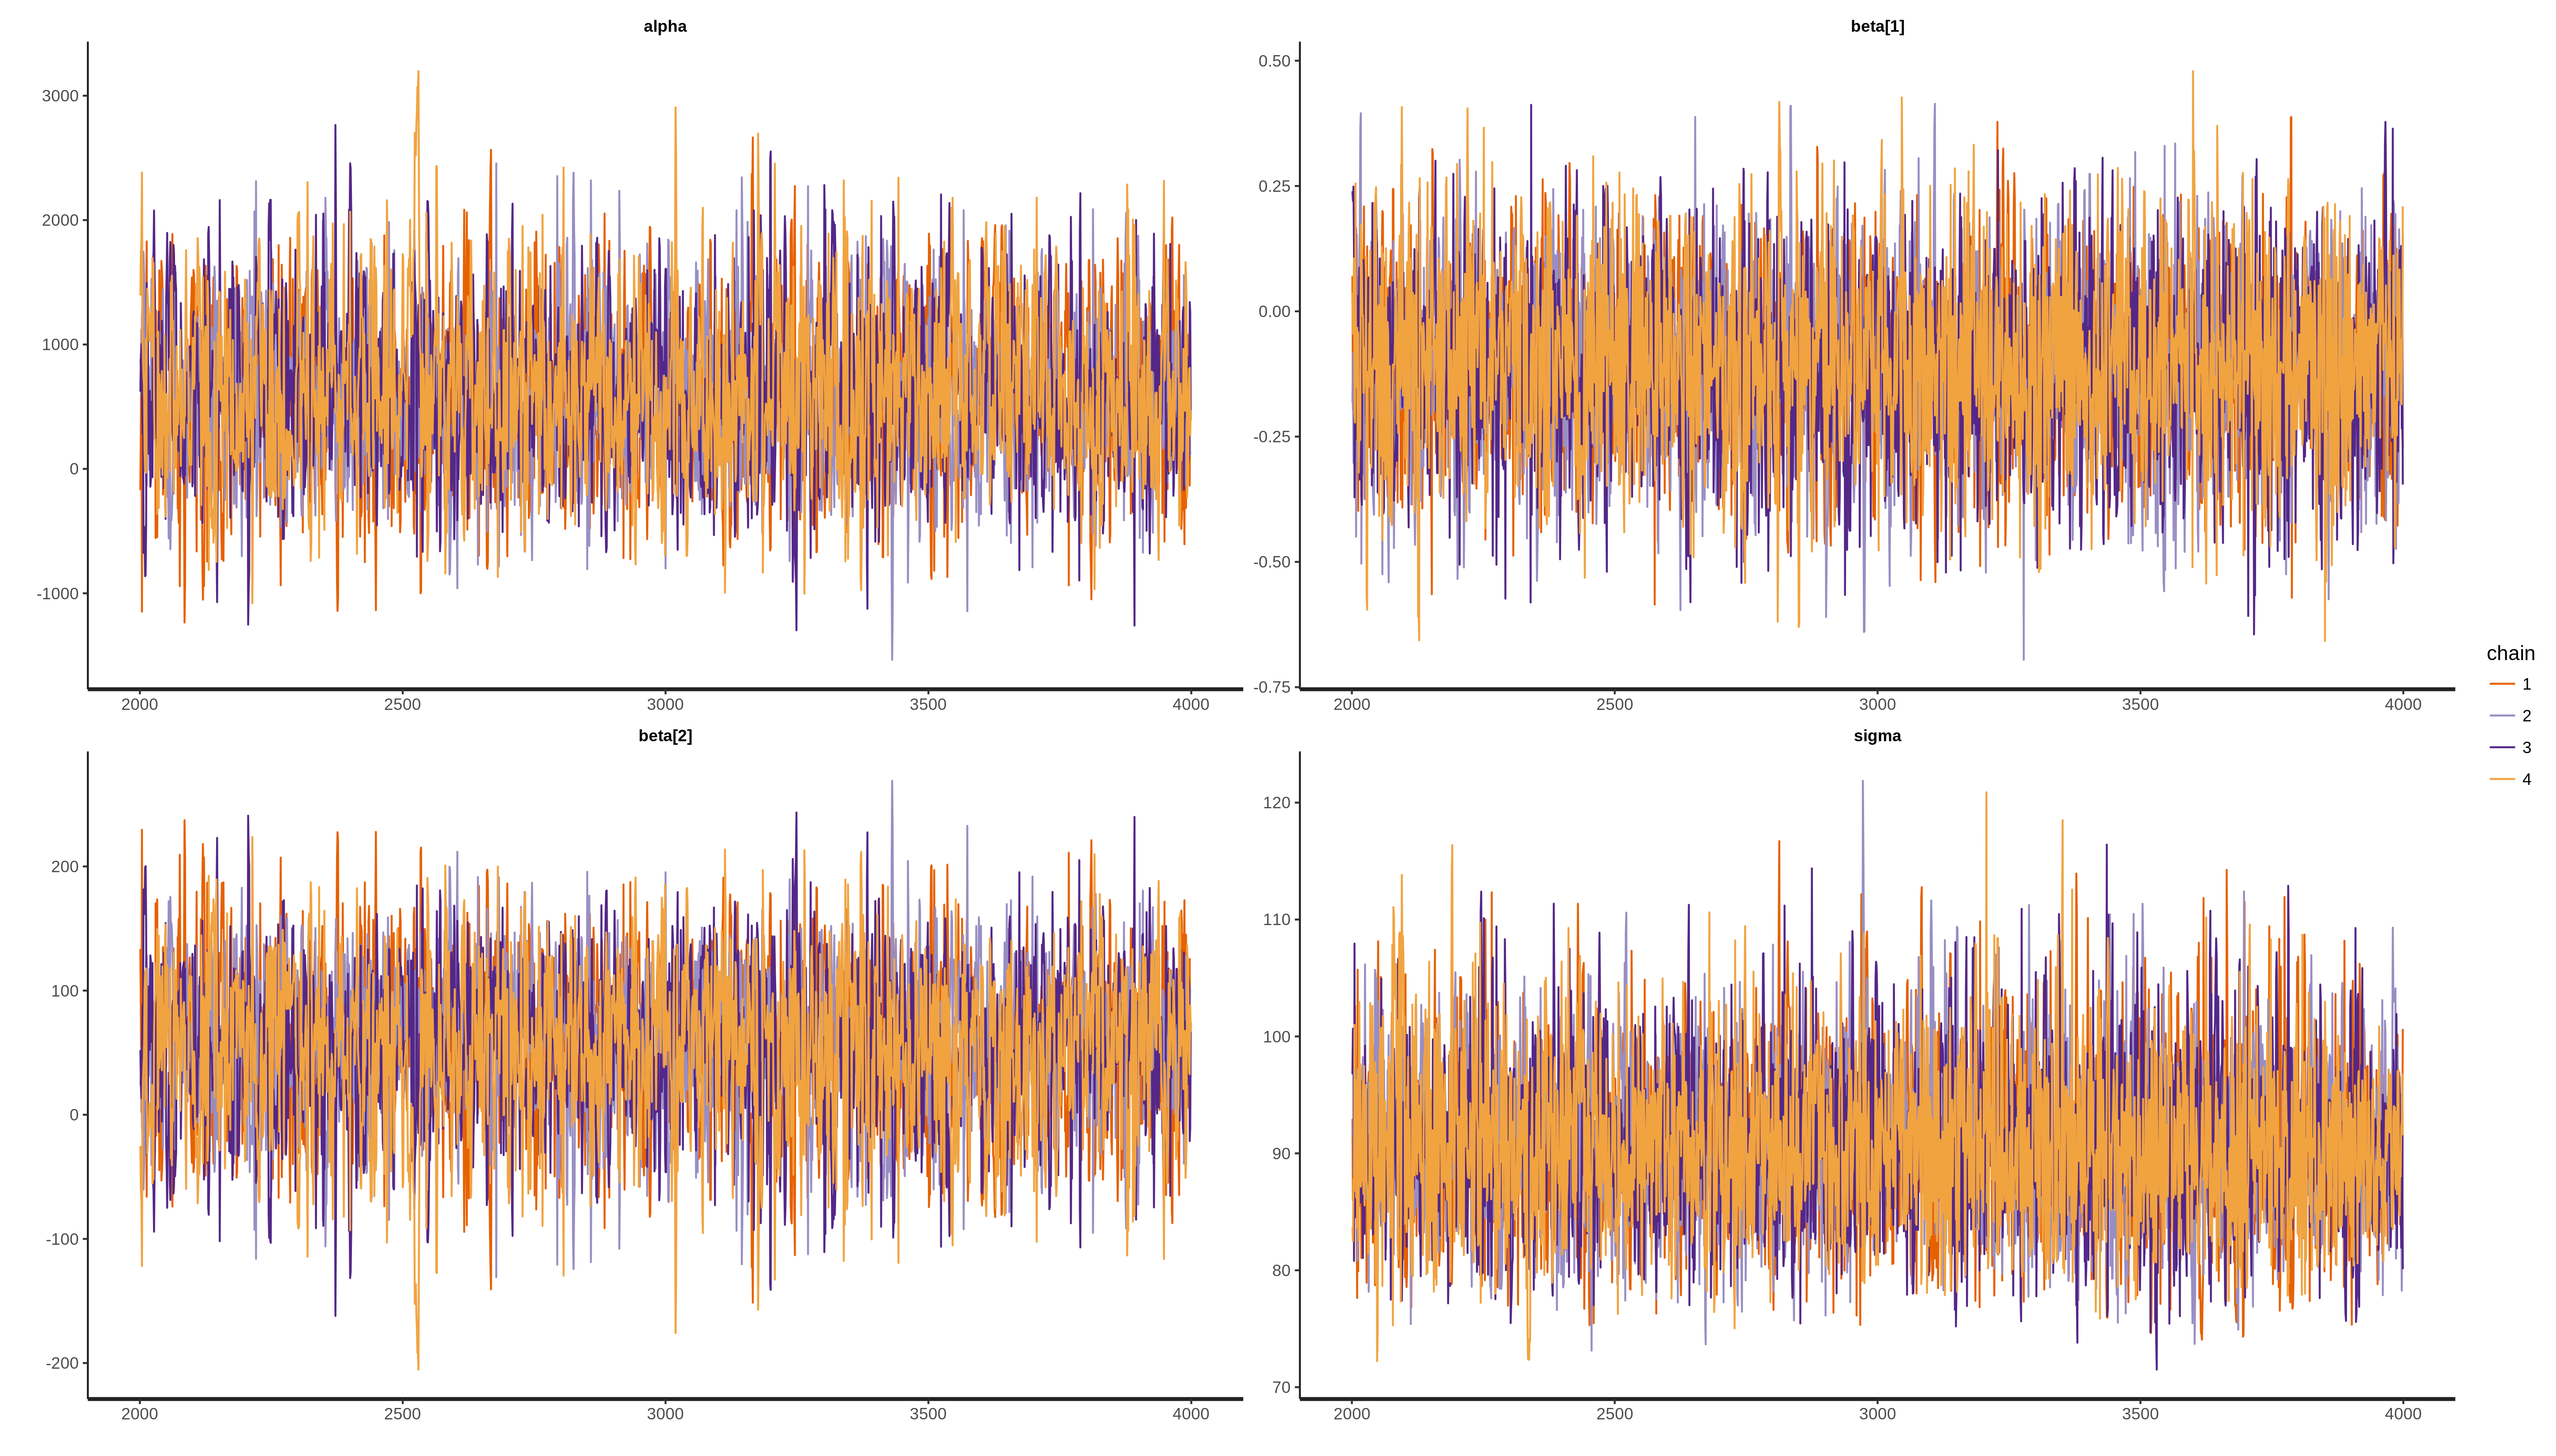
\includegraphics[width = 0.99\textwidth]{code/traceplot2.png}
\end{center}
\end{frame}

\begin{frame}[fragile]
\frametitle{Posterior Summaries}
{\tiny
\begin{verbatim}
> summary(regfit)$summary
                 mean      se_mean          sd         2.5%           25%
alpha    601.47469242 11.155331426 593.8138899 -490.6827947  191.95702515
beta[1]   -0.10907827  0.002090211   0.1628532   -0.4288071   -0.21721217
beta[2]   54.30721025  1.113999466  59.3528808  -67.0703765   16.13727134
beta[3]    0.02146048  0.001504924   0.1060208   -0.1860389   -0.05051183
sigma     90.81032505  0.088702720   6.7013775   78.7561024   86.06563171
lp__    -496.94003128  0.028859472   1.6090604 -500.9452935 -497.77083742
                  50%           75%        97.5%    n_eff      Rhat
alpha    570.66425923  9.840412e+02 1823.5656680 2833.582 1.0024421
beta[1]   -0.10911846  4.565740e-04    0.2095149 6070.329 1.0000127
beta[2]   57.29746473  9.525990e+01  163.6458877 2838.662 1.0024554
beta[3]    0.02158836  9.293641e-02    0.2261381 4963.105 0.9998738
sigma     90.37856417  9.514879e+01  105.0946718 5707.610 0.9998136
lp__    -496.63425539 -4.957597e+02 -494.7635700 3108.622 1.0010516
\end{verbatim}
}
Can also specify which parameters you want summaries of, e.g.
\verb0> summary(regfit, pars = c("beta"))$summary0
\end{frame}

\begin{frame}[fragile]
\frametitle{More Posterior Summaries}
\verb0lp__0: value of the log posterior at every iteration.\\
\verb0n_eff0: effective sample size.\\
\begin{itemize}
\item equivalent number of iid draw for that parameter.
\end{itemize}
\verb0Rhat0: potential scale reduction factor.
\begin{itemize}
\item convergence diagnostic based on multiple chains.
\item \verb0Rhat0 $< 1.01$: no evidence against convergence \emph{for that parameter}.\\~\\
\end{itemize}
\verb0shinystan0 \verb0R0 package:
\begin{itemize}
\item \url{http://mc-stan.org/interfaces/shinystan}\\~\\
\end{itemize}
Extract posterior draws into a named list:
\vspace{-0.2cm}
\tiny{
\begin{verbatim}
> regfitdraws <- extract(regfit)
> str(regfitdraws, 1)
List of 4
 $ alpha: num [1:8000(1d)] 1942.1 30.9 158.2 824.3 1634.2 ...
 $ beta : num [1:8000, 1:3] -0.278 -0.124 -0.1108 -0.1193 -0.0119 ...
 $ sigma: num [1:8000(1d)] 100.1 99 91.5 81.6 93.2 ...
 $ lp__ : num [1:8000(1d)] -499 -497 -495 -497 -497 ...
\end{verbatim}
}
\end{frame}


\begin{frame}[fragile]
\frametitle{Regression with Centered and Scaled Data}
Adapted from \verb0regression_cs.stan0.\\
\begin{columns}
\begin{column}{0.45\textwidth}
{\tiny
\begin{verbatim}
data {
  ...
}
transformed data {
  vector[n_obs] y_cs;
  matrix[n_obs, n_cov] x_cs;
  real y_mn;
  real<lower = 0> y_sd;
  vector[n_cov] x_mn;
  vector<lower = 0>[n_cov] x_sd;

  // center and scale y
  y_mn = mean(y);
  y_sd = sd(y);
  y_cs = (y - y_mn)/y_sd;

  // center and scale x
  for(i in 1:n_cov){
    x_mn[i] = mean(x[,i]);
    x_sd[i] = sd(x[,i]);
    x_cs[,i] = (x[,i] - x_mn[i]) / x_sd[i];
  }
}
parameters {
  real alpha_cs;
  vector[n_cov] beta_cs;
  real<lower = 0> sigma_cs;
}
\end{verbatim}
}
\end{column}
\begin{column}{0.55\textwidth}
This model is equivalent to \verb0regression.stan0 as long as:\\~\\
\begin{itemize}
\item We translate the priors on \verb0alpha0, \verb0beta0, and \verb0sigma0 into priors on their \verb0_cs0 versions.\\~\\
\item We transform back to \verb0alpha0, \verb0beta0, and \verb0sigma0 if that is what we want to do inference on.
\end{itemize}
\end{column}
\end{columns}
\end{frame}

\begin{frame}[fragile]
\frametitle{Carefully Taking Into Account Transformations}
From \verb0regression_cs.stan0 (see file for full text).
{\tiny
\begin{columns}
\begin{column}{0.45\textwidth}
\begin{verbatim}
transformed data {
  ...
  // center and scale y
  y_mn = mean(y);
  y_sd = sd(y);
  y_cs = (y - y_mn)/y_sd;

  // center and scale x
  for(i in 1:n_cov){
    x_mn[i] = mean(x[,i]);
    x_sd[i] = sd(x[,i]);
    x_cs[,i] = (x[,i] - x_mn[i]) / x_sd[i];
  }

  // priors on _cs parameters
  x_mnsd = x_mn ./ x_sd;
  beta_cs_prior_mn = x_sd * beta_prior_mn / y_sd;
  beta_cs_prior_sd = x_sd * beta_prior_sd / y_sd;
  alpha_cs_prior_loc = (alpha_prior_loc-y_mn)/y_sd;
  alpha_cs_prior_scale = alpha_prior_scale / y_sd;
  sigma_cs_prior_scale = sigma_prior_scale / y_sd;
}
\end{verbatim}
\end{column}
\begin{column}{0.55\textwidth}
\begin{verbatim}
parameters {
  real alpha_cs;
  vector[n_cov] beta_cs;
  real<lower = 0> sigma_cs;
}
model {
  y_cs ~ normal(alpha_cs + x_cs*beta_cs, sigma_cs);
  beta_cs ~ normal(beta_cs_prior_mn, beta_cs_prior_sd);
  alpha_cs ~ cauchy(alpha_cs_prior_loc + dot_product(x_mnsd, beta_cs), alpha_cs_prior_scale);
  sigma_cs ~ student_t(sigma_prior_df, 0, sigma_cs_prior_scale);
}
generated quantities {
  real alpha;
  vector[n_cov] beta;
  real<lower = 0> sigma;

  beta = (beta_cs ./ x_sd) * y_sd;
  alpha = alpha_cs * y_sd - dot_product(x_mn, beta) + y_mn;
  sigma = sigma_cs * y_sd;
}
\end{verbatim}
\end{column}
\end{columns}}
\vspace{.5cm}
Note: Transformed Data and Generated Quantities Blocks
\end{frame}


\begin{frame}[fragile]
\frametitle{Transformed data and parameters}
Transformed data: transform once before running MCMC.\\~\\

Transformed parameters: transform once per leapfrog step.\\~\\

For example:
\begin{columns}
\begin{column}{0.3\textwidth}
\end{column}
\begin{column}{0.7\textwidth}
{\tiny
\begin{verbatim}
data {
  ...
}
transformed data {
  vector[n_obs] log_y;
  log_y = log(y);
}
parameters {
  ...
}
transformed parameters {
  real<lower = 0> sigma;
  sigma = sqrt(sigma);
}
model {
  log_y ~ normal(mu, sigma);
  sigma2 ~ inv_gamma(a, b);
  ...
}
\end{verbatim}
}
\end{column}
\end{columns}
\end{frame}

\begin{frame}[fragile]
\frametitle{Other places to put transformations}
Model block:
\begin{itemize}
\item Computed once per leapfrog step --- useful for intermediate quantities you don't want MCMC draws for.
\item No constraints allowed here.
\end{itemize}
{\tiny
\begin{verbatim}
parameters {
  real mu;
  real<lower = 0> sigma2;
}
model {
  real sigma;
  sigma = sqrt(sigma2);
  log_y ~ normal(mu, sigma);
  ...
}
\end{verbatim}
}
Generated quantities block:
\begin{itemize}
\item Computed once per MCMC iter --- useful for quantities you want draws for, but aren't needed for computing the posterior.
\item Can also put random draws here, e.g. for predictive dists.
\item Constraints allowed, but not necessary.
\end{itemize}
{\tiny
\begin{verbatim}
model { ... }
generated quantities {
  real muoversigma;
  muoversigma = mu / sqrt(sigma2);
}
\end{verbatim}
}
\end{frame}

\begin{frame}[fragile]
\frametitle{Where should I put my transformation for max efficiency?}
\textbf{Transformed data block:}
\begin{itemize}
\item All pure functions of data, or other intermediate quantities that don't depend on parameters.\\~\\
\end{itemize}
\textbf{Transformed parameters block:}
\begin{itemize}
\item Quantities used on the RHS of sampling statements that you also want MCMC draws for.\\~\\
\end{itemize}
\textbf{Model block:}
\begin{itemize}
\item Intermediate quantities used on RHS of sampling statements.\\~\\
\end{itemize}
\textbf{Generated quantities block:}
\begin{itemize}
\item Quantities you want MCMC draws for that aren't already in the parameters or transformed parameters block.
\end{itemize}
\end{frame}

\begin{frame}[fragile]
\frametitle{All Possible Program Blocks}
Only the parameters and model blocks are mandatory,\\
but the blocks must appear in this order.
{\tiny
\begin{verbatim}
functions {
  // define user defined functions here (see manual)
}
data {
  // define all input (data / hyperparameter) variables here
}
transformed data {
  // create transformations of data and other intermediate
  // quantities that don't depend on parameters here
}
parameters {
  // define all model parameters here
}
transformed parameters {
  // create any needed transformations of parameters here
}
model {
  // create the log posterior density here
}
generated quantities {
  // create any other variables you want draws for here
}
\end{verbatim}}
\end{frame}

\begin{frame}[fragile]
\frametitle{Tricks for Better/Faster Samplers in Stan}
The centered and scaled model reduces fit time per chain from 3 minutes to 4 seconds.\\~\\

HMC/Stan works best when:
\begin{itemize}
\item All parameters are on similar scales.
\item Posterior geometries aren't ``weird''.
\begin{itemize}
\item Common in hierarchical models --- more later.
\end{itemize}
\end{itemize}
How to put parameters on the same scale.
\begin{itemize}
\item Center and scale responses and covariates.
\item Work on the log scale, e.g. \verb0logy ~ normal(.,.);0 is better than \verb0y ~ lognormal(.,.);0\\~\\
\end{itemize}

Centering and scaling data often drastically speeds up model fits because it makes adaptation easier.
\end{frame}

\begin{frame}[fragile]
\frametitle{Dealing with Hierarchical Models}
Example: same regression, now taking into account observation errors.\\~\\

Now we specify the model directly on centered and scaled $y_i$ and $\bm{x}_i'$:
\begin{align*}
y_i &\stackrel{ind}{\sim} \mathrm{N}(\theta_i, s_i^2),\\
\theta_i &\stackrel{ind}{\sim} \mathrm{N}(\alpha + \bm{x}_i'\bm{\beta}, \sigma^2),
\end{align*}
for $i=1,2,\dots,N$, where $s_i$ is the known observation SE for $y_i$.
\end{frame}

\begin{frame}[fragile]
\frametitle{Known Observation Error Variances in Stan}
From \verb0reg_error.stan0 (about 1 minute to fit):
{\scriptsize
\begin{verbatim}
data {
  int<lower = 1> n_obs;
  int<lower = 1> n_cov;
  vector[n_obs] y;
  vector<lower = 0>[n_obs] y_se;
  ...
}
transformed data {
  ...
  // note: have to convert y_se to y_cs_se
}
parameters {
  real alpha_cs;
  vector[n_cov] beta_cs;
  vector[n_obs] theta_cs;
  real<lower = 0> sigma_cs;
}
model {
  y_cs ~ normal(theta_cs, y_cs_se);
  theta_cs ~ normal(alpha_cs + x_cs*beta_cs, sigma_cs);
  beta_cs ~ normal(beta_prior_mn, beta_prior_sd);
  alpha_cs ~ cauchy(alpha_prior_loc, alpha_prior_scale);
  sigma_cs ~ student_t(sigma_prior_df, 0, sigma_prior_scale);
}
\end{verbatim}
}
\end{frame}

\begin{frame}[fragile]
\frametitle{Problems}
{\tiny
\begin{verbatim}
> regerrordat <- list(n_obs = n, n_cov = length(beta), y = y, x = x, y_se = ses,
+                     alpha_prior_loc = 0, alpha_prior_scale = 10,
+                     beta_prior_mn = 0, beta_prior_sd = 10,
+                     sigma_prior_df = 5, sigma_prior_scale = 10)
> regerrorfit0 <- stan("reg_error.stan", data = regerrordat, chains = 1, iter = 1)
> regerrorfit <- stan(fit = regerrorfit0, data = regerrordat, cores = 4, chains = 4,
                      warmup = 2000, iter = 4000, open_progress = FALSE)
Warning messages:
1: There were 119 divergent transitions after warmup. Increasing adapt_delta above 0.8 may help. See
http://mc-stan.org/misc/warnings.html#divergent-transitions-after-warmup
2: There were 4 chains where the estimated Bayesian Fraction of Missing Information was low. See
http://mc-stan.org/misc/warnings.html#bfmi-low
3: Examine the pairs() plot to diagnose sampling problems
\end{verbatim}}

\end{frame}

\begin{frame}[fragile]
\frametitle{Guide to Stan's Warnings}
Summarizing from \url{http://mc-stan.org/misc/warnings.html}\\~\\

Exception ... Hamiltonian proposal rejected: {\tiny\verb9Exception thrown at line 37: normal_log: Scale parameter is 0, but must be > 0!9}.
\begin{itemize}
\item Not a problem if the proportion of iters with exceptions is low.
\item If the proportion is high: indication of a problem w/ the model.\\
\begin{itemize}
\item[] e.g. maybe a hierarchical variance should be zero.\\~\\
\end{itemize}
\end{itemize}

Low Bayesian Fraction of Missing Information (BFMI):
\begin{itemize}
\item Indicates that the adaptation turned out poorly and the chain did not properly explore the posterior.
\item Can solve by increasing \verb0warmup0 or reparameterizing.
\end{itemize}
\end{frame}

\begin{frame}[fragile]
\frametitle{Focus on Divergent Transitions}
Divergent transitions after warmup: {\tiny\verb61: There were 119 divergent transitions after warmup. Increasing adapt_delta above 0.8 may help.6}
\vspace{-0.4cm}
\begin{itemize}
\item Indicates that geometric ergodicity is breaking down. \textbf{\emph{Just one divergent transition is enough to be concerning.}}
\item Can solve via increasing \verb0adapt_delta0:\\
\verb0stan(..., control = list(adapt_delta = .99))0\\~\\
\end{itemize}

\verb0adapt_delta0 is the target Metropolis acceptance rate, which is controlled via the leapfrog step size.\\~\\

Lowering the leapfrog step size forces the numerical integrator to follow the local curvature of the target distribution more closely...\\~\\

But this doesn't always work! Common in hierarchical models!
\end{frame}

\begin{frame}[fragile]
\frametitle{The Problem with Hierarchical Models}
Good discussion in \textbf{HMC for Hierarchical Models}: \url{https://arxiv.org/pdf/1312.0906.pdf}\\~\\

In a nutshell: these posterior distributions have weird geometries.
\begin{itemize}
\item Parameters are highly correlated, and global and local correlations may be very different.
\item Gibbs samplers have high autocorrelation.
\item Random Walk Metropolis samplers have small step sizes.
\item HMC more likely to have divergent transitions.
\item Geometric ergodicity often fails \textbf{\emph{using any method}}.\\~\\
\end{itemize}
How to fix this?
\begin{itemize}
\item Gibbs: \textbf{reparameterize}, parameter expansion, interweaving.
\item HMC: \textbf{reparameterize}, decrease step size, Riemannian HMC.
\end{itemize}
\end{frame}

\begin{frame}[fragile]
\frametitle{Centered vs. noncentered parameterizations}
\begin{align*}
y_i &\stackrel{ind}{\sim}\mathrm{N}(\theta_i, s_i^2) && \theta_i \stackrel{ind}{\sim} \mathrm{N}(\alpha + \bm{x}_i'\bm{\beta}, \sigma^2); && \mbox{(centered)}\\
y_i &\stackrel{ind}{\sim} \mathrm{N}(\alpha + \bm{x}_i'\bm{\beta} + \sigma\varepsilon_{i}, s_i^2), && \varepsilon_i \stackrel{iid}{\sim} \mathrm{N}(0, 1). && \mbox{(noncentered)}\\
\end{align*}
Define the signal-to-noise ratio: $\sigma^2/\overline{s}^2$.\\~\\

Centered parameterization:
\begin{itemize}
\item Usually the natural way to write the model.
\item Results in easy MCMC when the signal-to-noise ratio is large.\\~\\
\end{itemize}
Noncentered parameterization:
\begin{itemize}
\item Usually found by centering and scaling: $\varepsilon_i = (\theta_i - \alpha - \bm{x}_i'\bm{\beta})/\sigma$.
\item Results in easy MCMC when the signal-to-noise ratio is small.
\end{itemize}
\end{frame}

\begin{frame}[fragile]
\frametitle{Noncentered Regression with Observation Errors}
From \verb0reg_error_nc.stan0 (about 30 seconds per chain):\\~\\
{\tiny
\begin{verbatim}
parameters {
  real alpha_cs;
  vector[n_cov] beta_cs;
  vector[n_obs] theta_cs_raw;
  real<lower = 0> sigma_cs;
}
transformed parameters{
  vector[n_obs] theta_cs;
  theta_cs = theta_cs_raw*sigma_cs + alpha_cs + x_cs*beta_cs;
}
model {
  y_cs ~ normal(theta_cs, y_cs_se);
  theta_cs_raw ~ normal(0, 1);
  beta_cs ~ normal(beta_prior_mn, beta_prior_sd);
  alpha_cs ~ cauchy(alpha_prior_loc, alpha_prior_scale);
  sigma_cs ~ student_t(sigma_prior_df, 0, sigma_prior_scale);
}
\end{verbatim}}
No divergent transitions or low BFMI with this parameterization.
\end{frame}

\begin{frame}[fragile]
\frametitle{Stan vs Gibbs for Hierarchical Models}
Stan's major advantages:
\begin{itemize}
\item Gibbs fails in high dimensions.
\item Stan tends to let you know when geometric ergodicity fails.
\item Stan tends to be more efficient.
\end{itemize}
\begin{center}
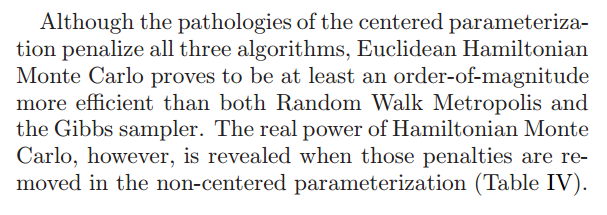
\includegraphics[width = 0.4\textwidth]{center.png}\\
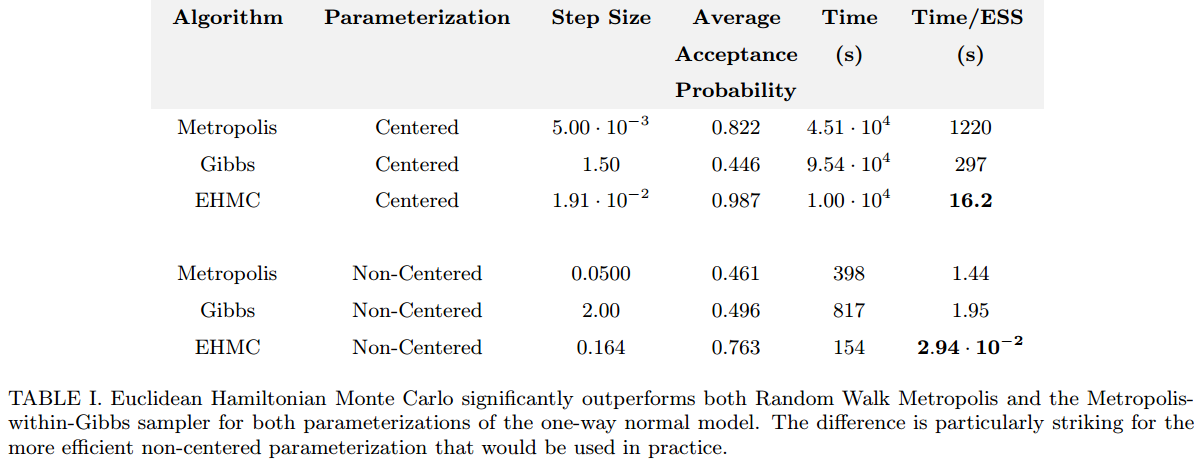
\includegraphics[width = 0.8\textwidth]{hmctable.png}
\end{center}
From \textbf{HMC for Hierarchical Models}: \\
\ \ \ \ \ \url{https://arxiv.org/pdf/1312.0906.pdf}
\end{frame}

\begin{frame}[fragile]
\frametitle{Coming Soon: Riemannian HMC (and more)}
Good Riemannian HMC deals with all of this without user input.\\~\\

Momentum distribution $\bm{p}|\bm{q} \sim \mathrm{N}(\bm{0}, \bm{M}(\bm{q}))$.\\~\\
Setting $\bm{M}$ to a function of the Hessian of $\log {\color{blue}\pi(\bm{q})}$ works well.\\
 $\implies$ need second order \verb0autodiff0. They're working on it:\\~\\

\begin{center}
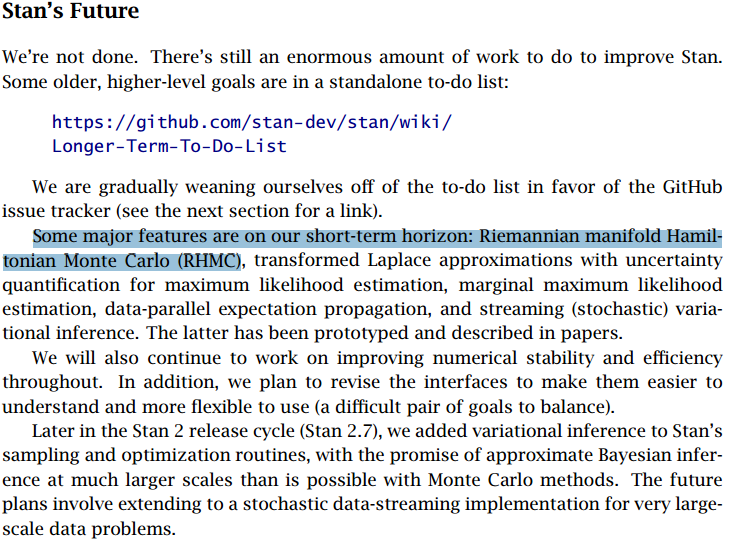
\includegraphics[width=0.5\textwidth]{stanfuture.png}
\end{center}
\end{frame}

\begin{frame}
      \begin{center}

        \font\endfont = cmss10 at 20.40mm
        \color{Red}
        \endfont
        \baselineskip 20.0mm

        Thank you!\\~\\

        Questions?

      \end{center}
\vspace{.4cm}
Matthew Simpson \hfill themattsimpson@gmail.com
\end{frame}
\end{document}

